\documentclass[../mathNotesPreamble]{subfiles}

\begin{document}
%  \relscale{1.4} %TODO
  \section{2.1: Visualizing Variation in Numerical Data}
  \begin{defn*}
    The \textbf{distribution of a sample} of data is a way of organizing the data by recording the
    \begin{itemize}
      \item values that were observed, and
      \item the frequencies of these values.
    \end{itemize}
  \end{defn*}
  
  \begin{ex*}
    Below are the number of goals scored by first year NCAA female soccer players in Division III in the 2016-17 season:
    \[11, 14, 16, 13, 13, 10, 13, 11, 16, 21, 13, 19, 10, 10, 14, 13, 10, 13, \]
    \[15, 10, 15, 13, 11, 19, 11, 11, 16, 10, 12, 11, 14, 11, 10, 14, 10, 19, 12\]
  \end{ex*}
  \vspace*{\stretch{1}}
  \noindent
  The \textbf{distribution} lists the values \emph{and} the frequencies:
  \begin{flushright}
    \begin{tabular}{@{}cc@{}}\toprule
      Value & Frequency \\\midrule
      10 & 8 \\
      11 & 7 \\
      12 & 2 \\
      13 & 7 \\
      14 & 4 \\
      15 & 2 \\
      16 & 3 \\
      17 & 0 \\
      18 & 0 \\
      19 & 3 \\
      20 & 0 \\
      21 & 1 \\\bottomrule
    \end{tabular}
  \end{flushright}
  \pagebreak

  \noindent
  A \textbf{dotplot} represents the data by using a dot where each value occurs:
  \begin{center}
    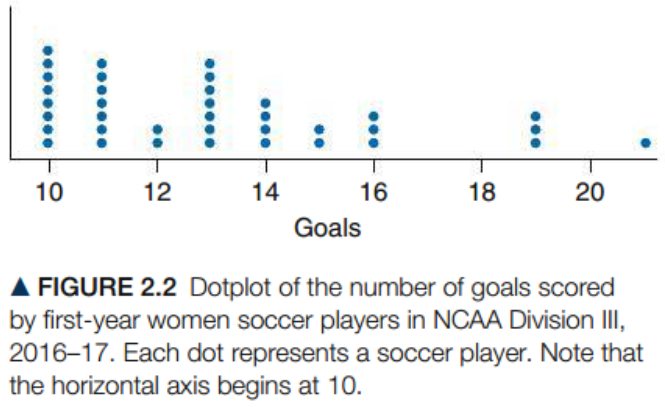
\includegraphics[width=0.5\linewidth]{images/math211_figure_2p02}
  \end{center}
  \vspace*{\stretch{1}}
  
  \section*{Histograms:}
  \noindent
  A \textbf{histogram} represents the data by using bars to indicate how much data lies in each \emph{bin} (also called \emph{interval} or \emph{class}):
  \begin{center}
    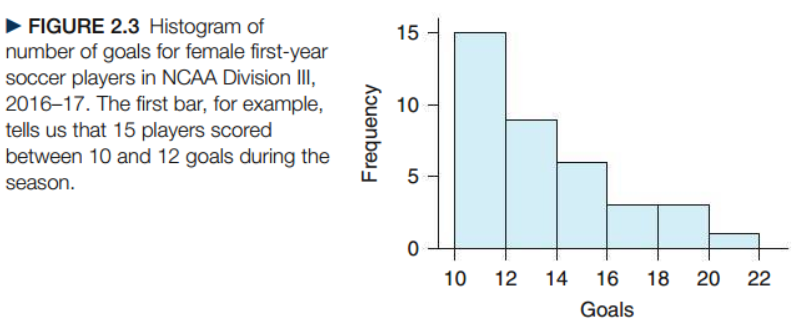
\includegraphics[width=0.65\linewidth]{images/math211_figure_2p03}
    \fbox{\parbox{0.7\linewidth}{\hspace*{\stretch{1}}Q: Where do we place data points that lie on a boundary?\hspace*{\stretch{1}}}}
  \end{center}
  \vspace*{\stretch{1}}
  \pagebreak
  
  \emph{Note:} Bin size plays a significant role in how the data is represented in a histogram. A bin width that is:
  \begin{itemize}
    \item too narrow shows too much detail.
    \item too wide hides detail.
  \end{itemize}
  \begin{center}
    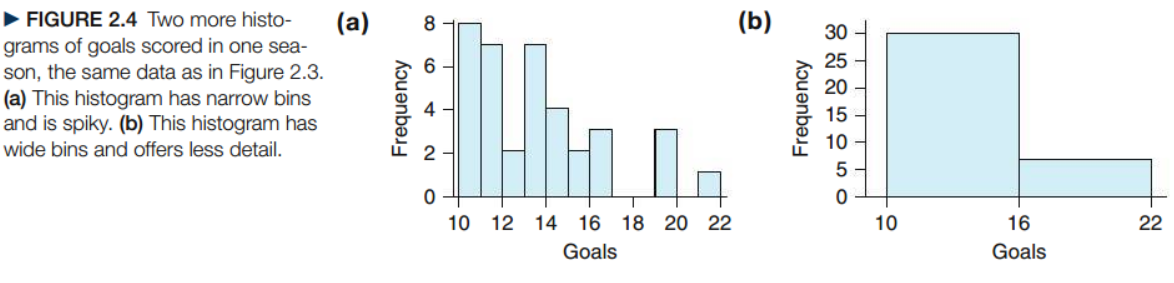
\includegraphics[width=0.85\linewidth]{images/math211_figure_2p04}
  \end{center}
  \vspace*{\stretch{1}}
  A \textbf{relative frequency histogram} changes the units on the vertical axis to represent relative frequencies:
  \begin{center}
    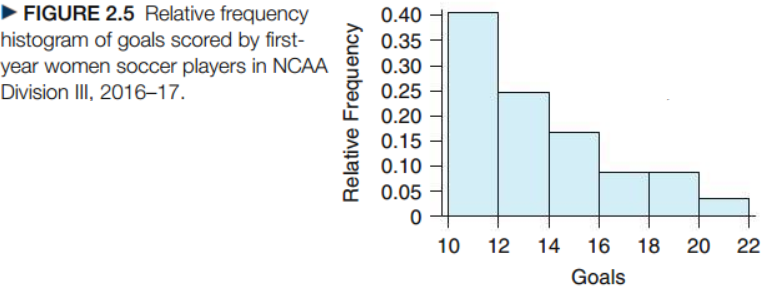
\includegraphics[width=0.65\linewidth]{images/math211_figure_2p05}
  \end{center}
  \vspace*{\stretch{1}}
  \pagebreak
  
  \section*{Stemplots:}
  \begin{defn*}
    A \textbf{stemplot} divides each observation into a \emph{stem} and \emph{leaf}. The \textbf{leaf} is the last digit in the observation, and the \textbf{stem} contains all the digits preceding the leaf.
  \end{defn*}
  \begin{ex*}
    A collection of college students who said that they drink alcohol were asked how many alcoholic drinks they had consumed in the last seven days. Their answers were:
    \[1, 1, 1, 1, 1, 2, 2, 2, 3, 3, 3, 3, 3, 4, 5, 5, 5, 6, 6, 6, 8, 10, 10, 15, 17, 20, 25, 30, 30, 40\]
  \end{ex*}
  \begin{center}
    \begin{tabular}{@{}ll@{}}\toprule
      Stem& Leaves\\\midrule
      0& 111112223333345556668\\
      1& 0057\\
      2& 05\\
      3& 00\\
      4& 0\\\bottomrule
    \end{tabular}
  \end{center}
  \vspace*{\stretch{1}}
  
  \begin{ex*}
    Below is a stemplot for exam grades. How many grades are between 40\% and 59\%?
  \end{ex*}
  \begin{center}
    \begin{tabular}{@{}ll@{}}\toprule
      Stem& Leaves\\\midrule
      3& 8\\
      4& \\
      5& \\
      6& 0257\\
      7& 00145559\\
      8& 0023\\
      9& 0025568\\
      10& 00\\\bottomrule
    \end{tabular}
  \end{center}
  \vspace*{\stretch{1}}

  \pagebreak
\end{document}
